\chapter{Instalación y configuración de \gls{CALDERA}} \label{caldera-conf}

\vspace{-2mm}

Como se ha comentado anteriormente, \gls{CALDERA} es un \textit{framework} desarrollado por MITRE basado en el marco de técnicas, tácticas y procedimientos de \texttt{MITRE \gls{ATT&CK}}. Este permite la simulación de adversarios complejos utilizando agentes distribuidos que pueden ejecutar una serie de técnicas descritas en el marco \gls{ATT&CK} para evaluar la robustez de la seguridad de una red o un \textit{host}. La principal ventaja de este \textit{framework} frente a otros reside en su capacidad de integrar múltiples \textit{plugins} y módulos que extienden sus funcionalidades, proporcionando la posibilidad de personalizar las operaciones de simulación de amenazas según necesidades específicas.


\subsubsection{Instalación de \gls{CALDERA}}

Para descargar \gls{CALDERA}, es necesario acceder al repositorio oficial de GitHub \cite{caldera}. Simplemente se clonará el repositorio activando la opción de copia recursiva en la máquina Kali por medio del siguiente comando:


\begin{center}
    \footnotesize
    \begin{mdframed}
            \begin{minted}{bash}
git clone https://github.com/mitre/caldera.git --recursive
        \end{minted}
    \end{mdframed}
\end{center}

\begin{figure}[H]
    \centering
    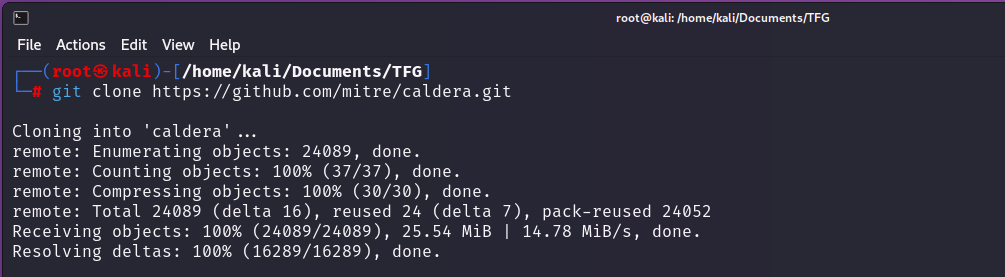
\includegraphics[width=1\linewidth]{imagenes/clone-caldera.png}
    \caption{Clonación del repositorio de CALDERA en la máquina atacante}
    \label{fig:git-caldera}
\end{figure}

A continuación, accedemos al directorio e instalamos las dependencias de \texttt{Python} por medio del siguiente comando:

\begin{center}
    \footnotesize
    \begin{mdframed}
            \begin{minted}{bash}
                            cd caldera
                    pip install -r requirements.txt
    \end{minted}
    \end{mdframed}
\end{center}

\vspace{-4mm}

\begin{figure}[H]
    \centering
    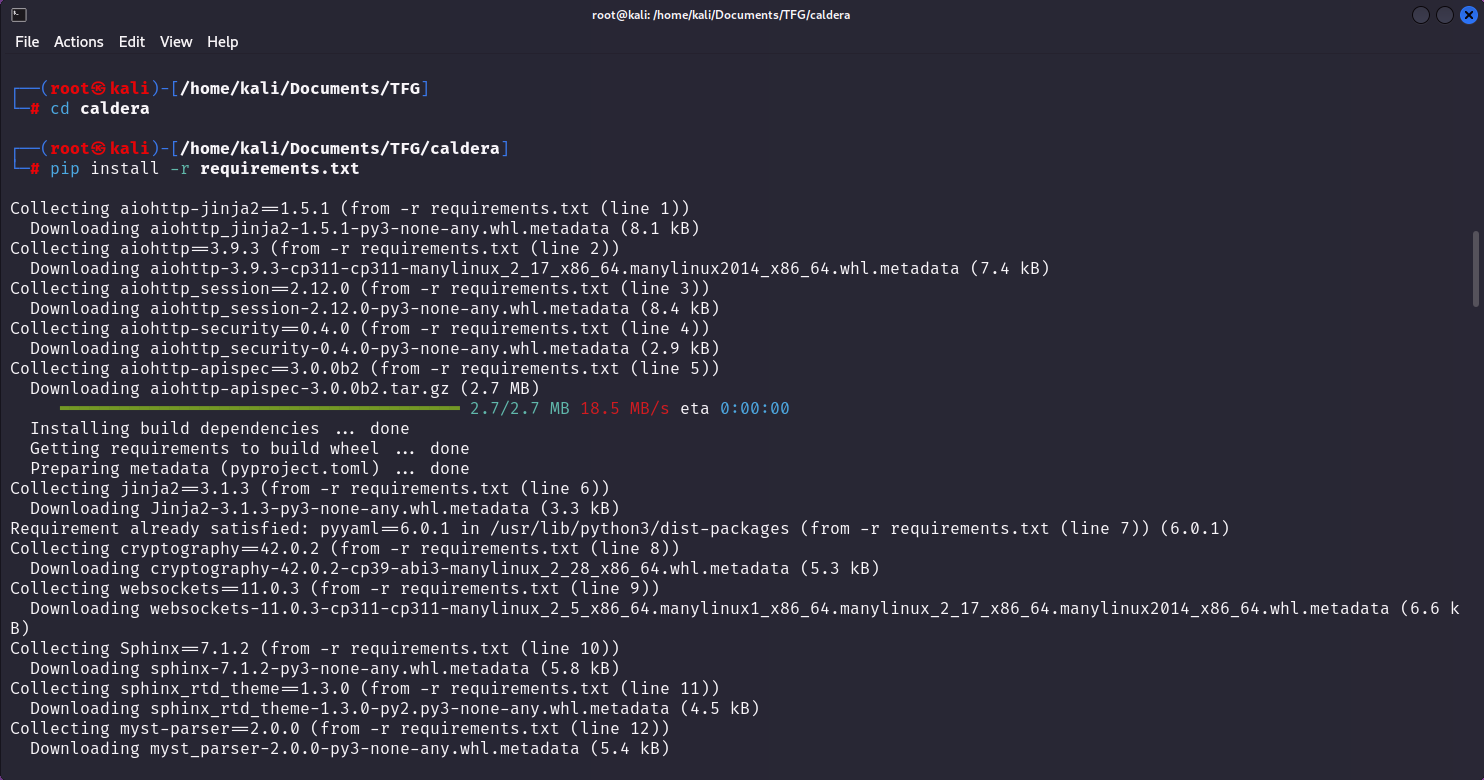
\includegraphics[width=1\linewidth]{imagenes/pip-install-requirements.png}
    \caption{Instalación de dependencias utilizadas por CALDERA}
    \label{fig:install-requirements}
\end{figure}

Por último, es necesario ejecutar el comando que levanta el servicio en el puerto 8888:

\begin{center}
    \footnotesize
    \begin{mdframed}
            \begin{minted}{javascript}
python server.py --build 
            \end{minted}
    \end{mdframed}
\end{center}

\vspace{-4mm}

\begin{figure}[H]
    \centering
    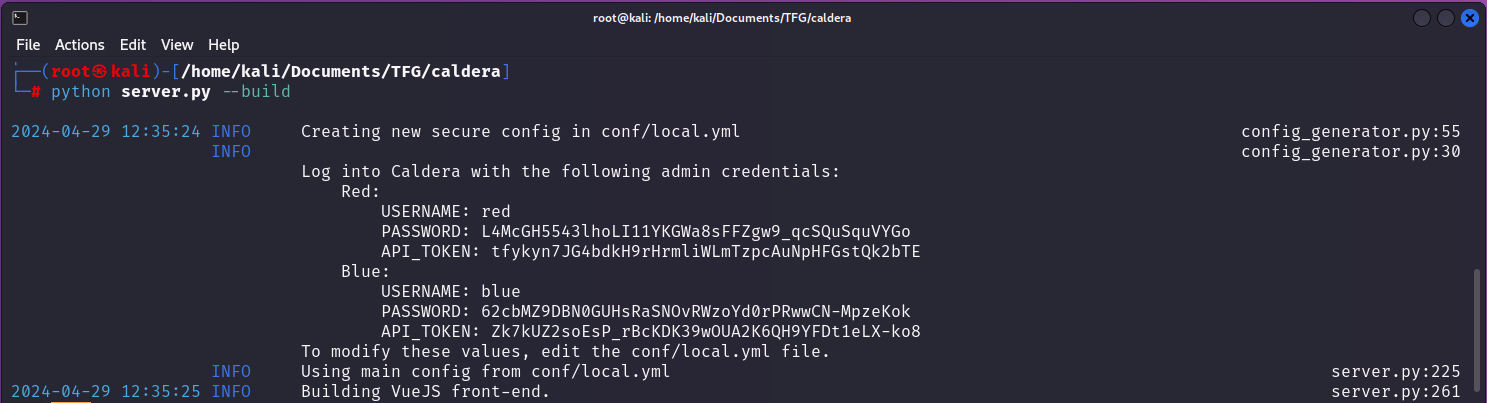
\includegraphics[width=1\linewidth]{imagenes/build-caldera.png}
    \caption{Ejecución del comando para levantar el servicio de \gls{CALDERA}}
    \label{fig:build_caldera-1}
\end{figure}

\newpage

\begin{figure}[H]
    \centering
    
    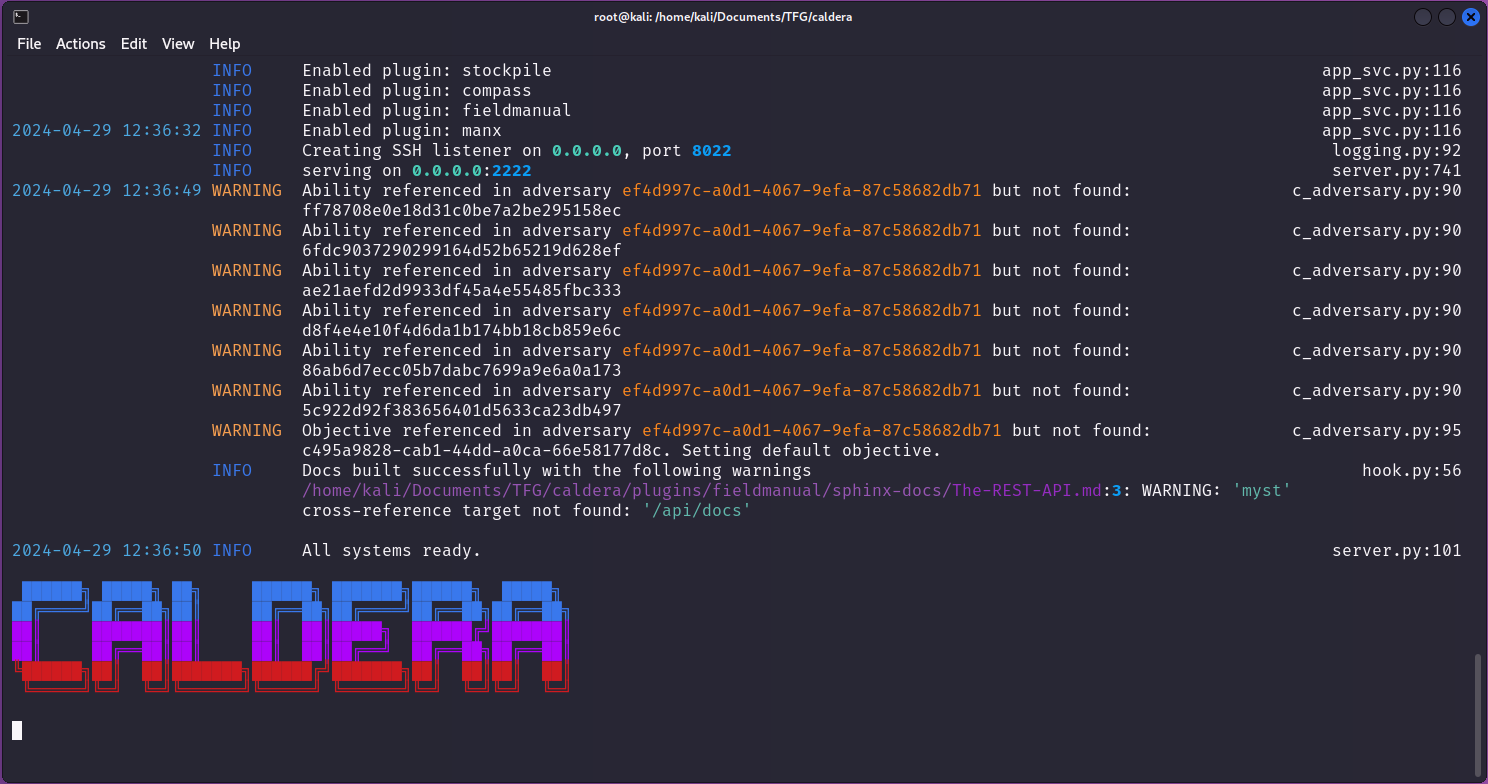
\includegraphics[width=1\linewidth]{imagenes/build-caldera-2.png}
    \caption{Ejecución del comando para levantar el servicio de \gls{CALDERA} (II)}
    \label{fig:build-caldera-2}
\end{figure}

Además de abrir el puerto \texttt{8888} para la interfaz web, también tiene habilitados los puertos \texttt{2222} y \texttt{8022} para el servicio de \gls{SSH}, que será posteriormente utilizado por los agentes como Sandcat para realizar operaciones de \gls{C2} \cite{calderaSSHTunneling}. \\

Una vez el servicio está corriendo, simplemente basta con acceder a través de un navegador a la interfaz de \texttt{localhost:8888/login} e iniciar sesión a través de las credenciales por defecto, a las cuales se puede acceder a través de la ruta \texttt{caldera/conf/default.yml}:

\begin{figure}[H]
    \centering
    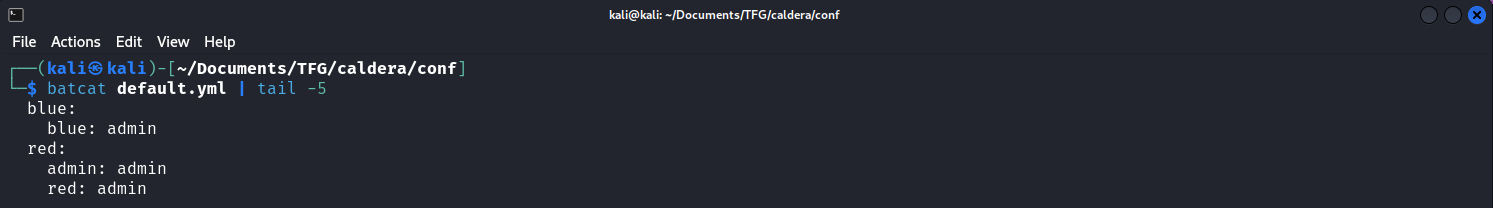
\includegraphics[width=1\linewidth]{imagenes/caldera-credentials.png}
    \caption{Fichero con credenciales por defecto de CALDERA}
    \label{fig:caldera-credentials}
\end{figure}

\begin{figure}[H]
    \centering
    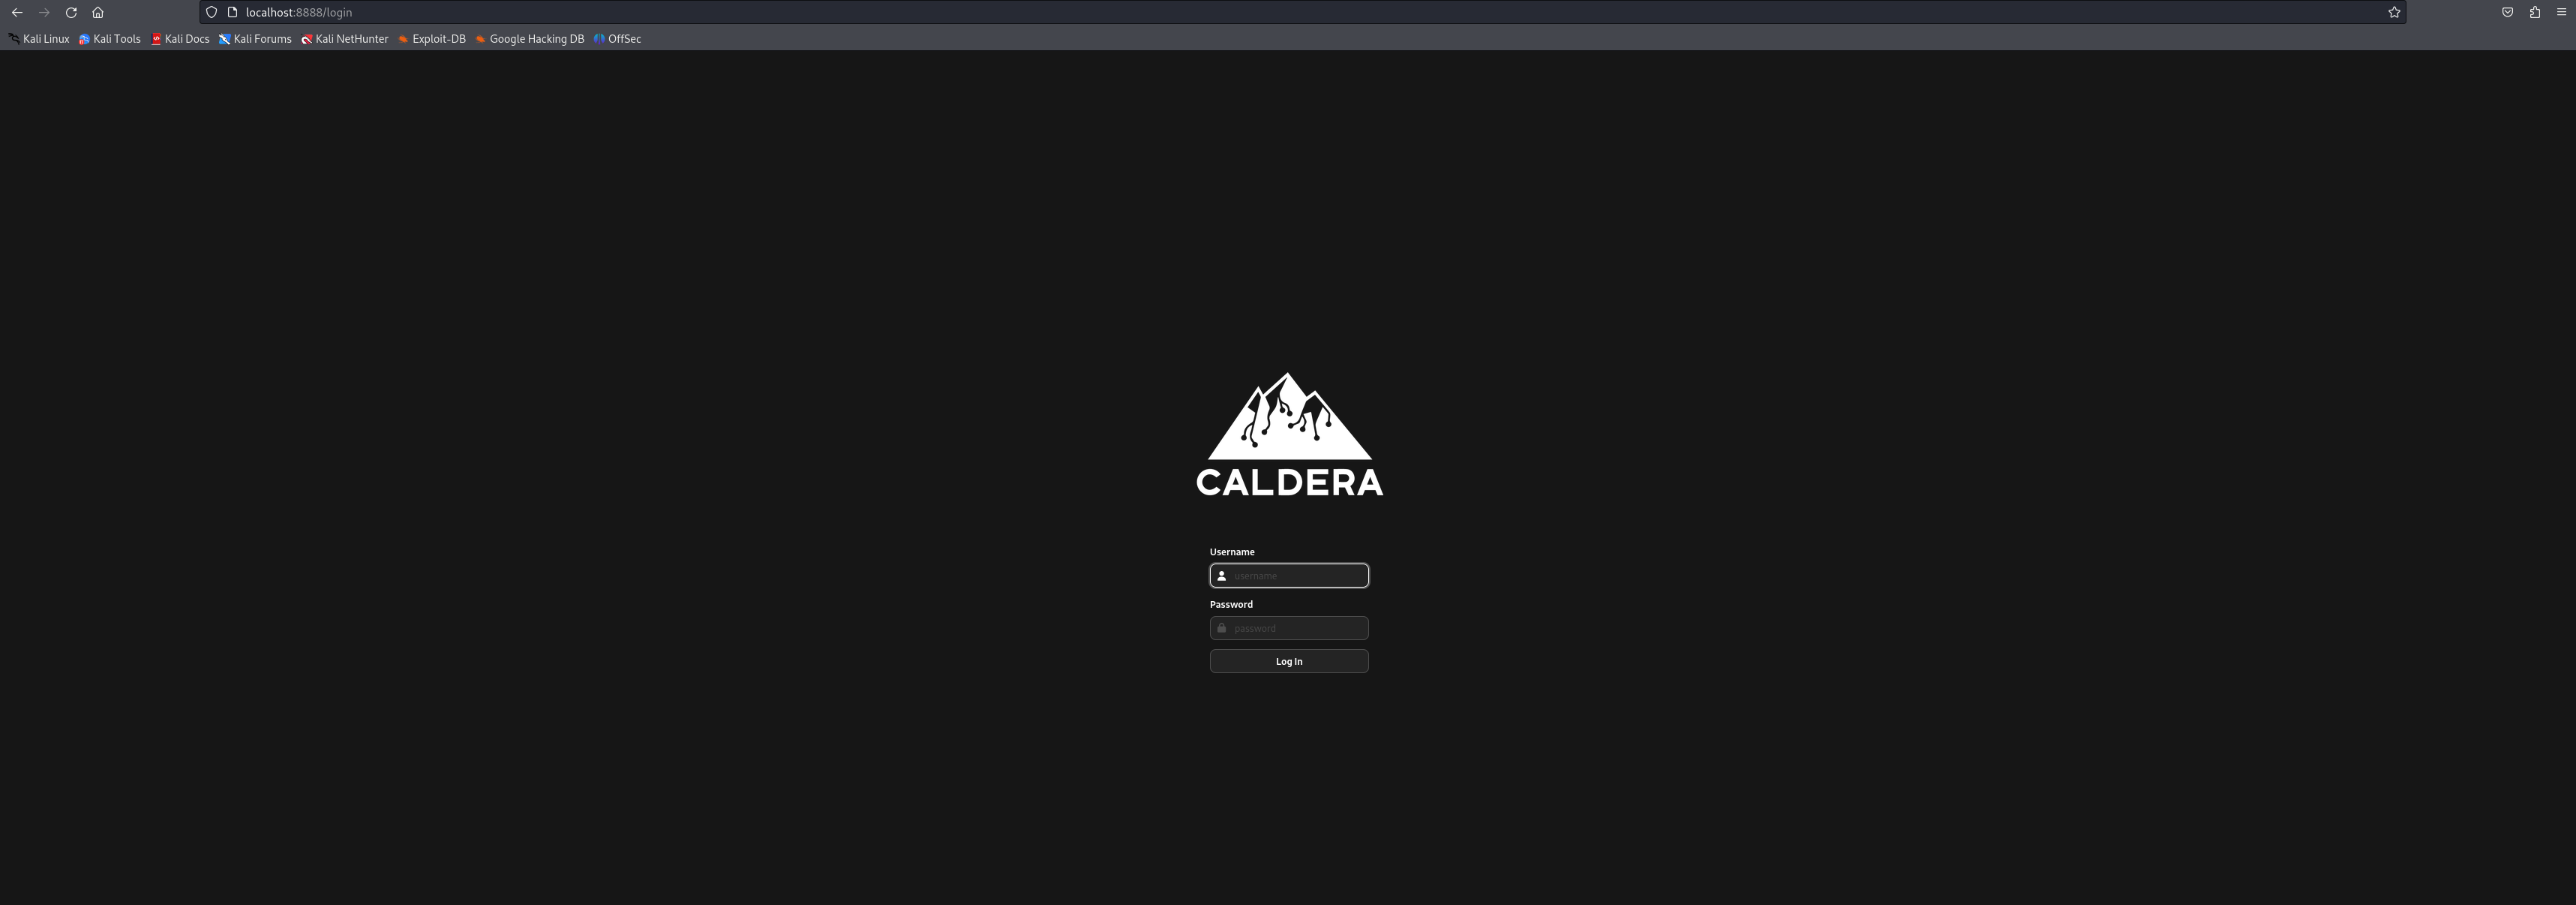
\includegraphics[width=1\linewidth]{imagenes/login-caldera.png}
    \caption{Pestaña de Inicio de sesión del \textit{framework}}
    \label{fig:login-caldera}
\end{figure}

\subsubsection{Configuración de \gls{CALDERA}}

Una vez se ha iniciado sesión, aparece una \textit{dashboard} con un panel de navegación a la izquierda. Este contiene cuatro secciones, tal y como se aprecia en la Tabla \ref{tab:caldera-sections}:

\begin{table}[H]
\centering
\footnotesize
\begin{tabularx}{\textwidth}{|X|X|}
\hline
\rowcolor{graylight}\texttt{Sección} & \texttt{Descripción} \\
\hline
\textbf{Campañas} & Permite a los usuarios crear y gestionar diferentes simulaciones de ataques, ajustando escenarios y monitorizando el progreso en tiempo real. \\
\hline
\textbf{Plugins} & Ofrece acceso a extensiones que pueden ser incorporadas para expandir la funcionalidad de CALDERA, incluyendo nuevas capacidades de inteligencia y herramientas de ataque. \\
\hline
\textbf{Configuración} & Permite a los administradores ajustar objetivos, contactos y archivos exfiltrados, así como gestionar cuentas de usuario. \\
\hline
\textbf{Recursos} & Proporciona enlaces a documentación, tutoriales y otros materiales de apoyo, así como herramientas de ofuscación de los \textit{payloads}. \\
\hline
\end{tabularx}
\caption{Descripción de las secciones principales en la interfaz de CALDERA}
\label{tab:caldera-sections}
\end{table}


\begin{figure}[H]
    \centering
    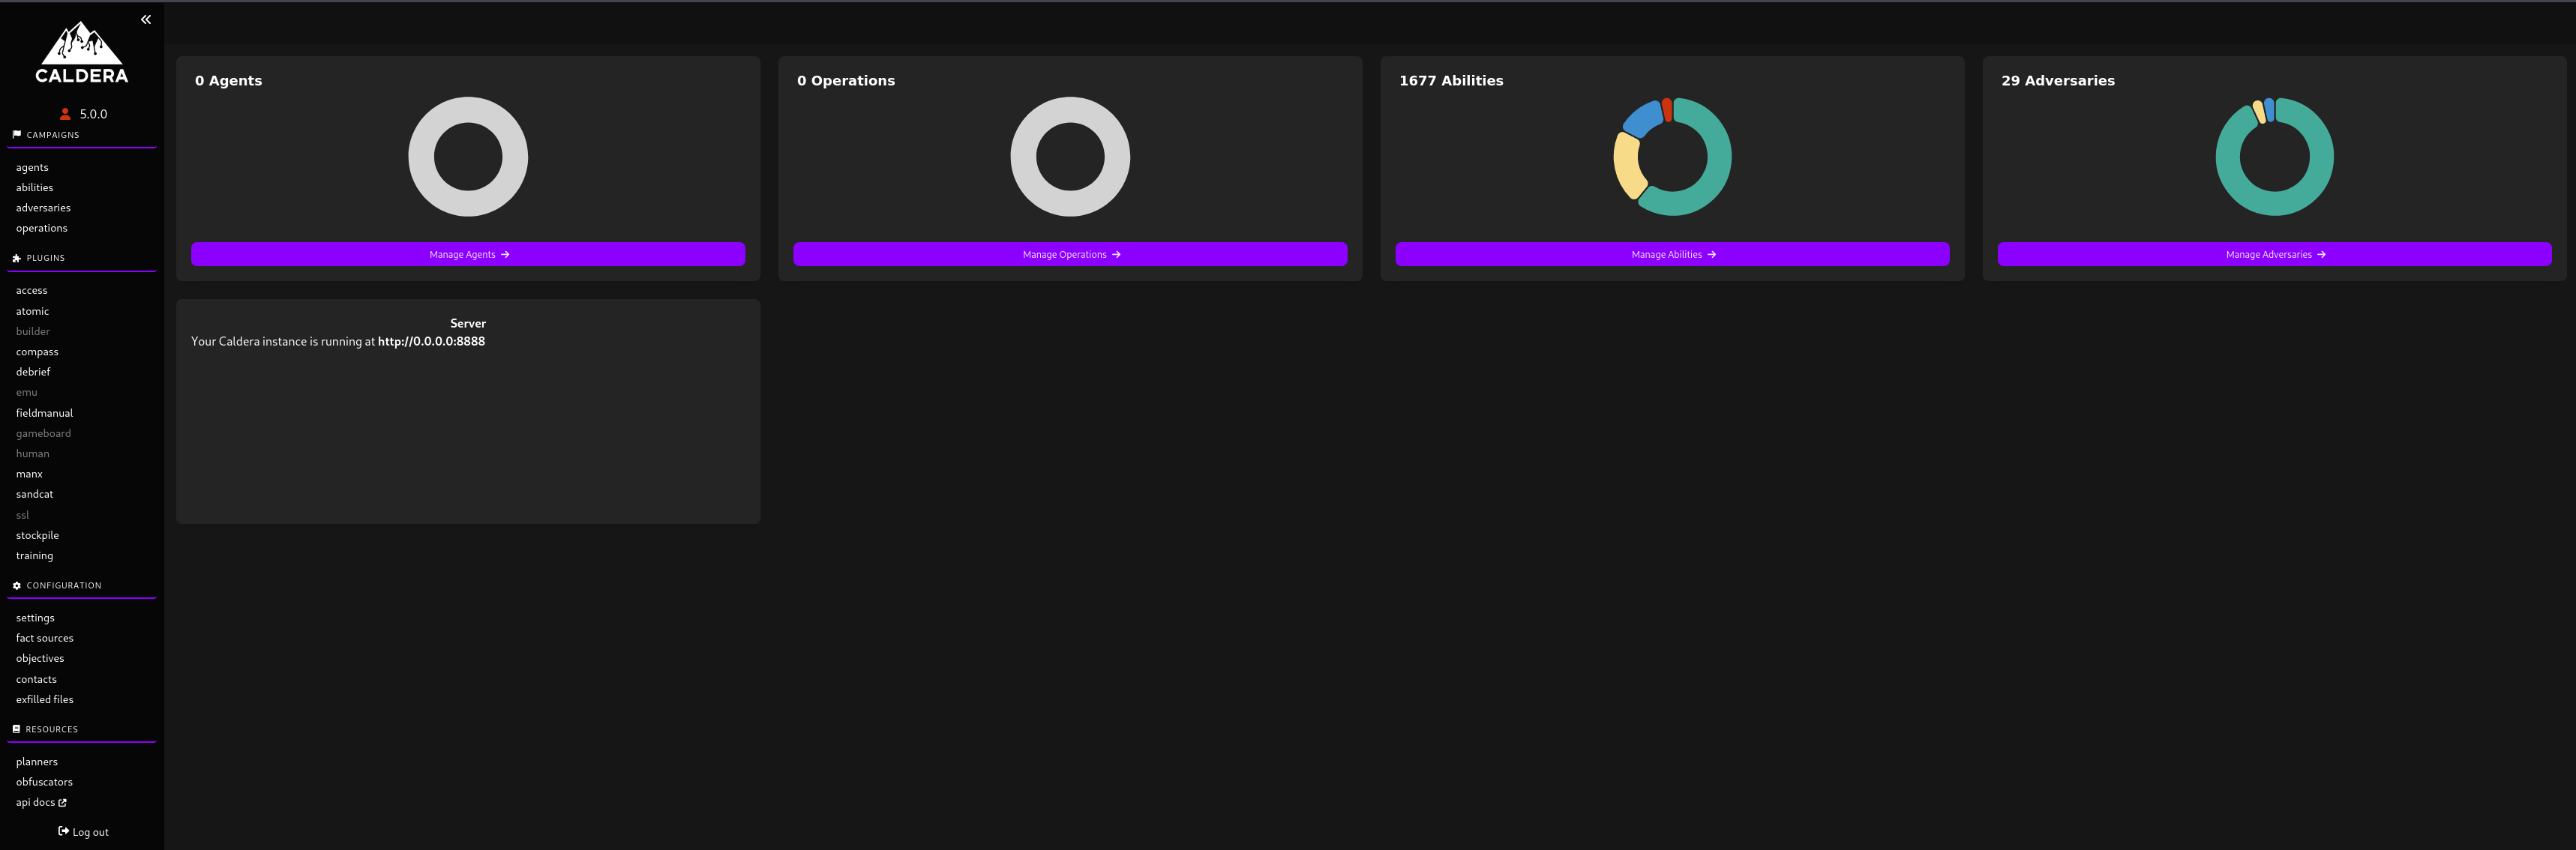
\includegraphics[width=1\linewidth]{imagenes/caldera-dashboard.png}
    \caption{Dashboard de la interfaz web del \textit{framework}}
    \label{fig:enter-label}
\end{figure}

Por otro lado, en el menú principal hay una serie de gráficas que referencian los cuatro elementos del \textit{framework} utilizados para efectuar la simulación de los ataques, como son los agentes, operaciones, habilidades y adversarios. Inicialmente el numero de agentes y operaciones está inicializado a cero, ya que estos deben de ser generados manualmente. 

Se comenzará creando un agente. Para ello es necesario acceder a su sección en la barra de navegación lateral y posteriormente hacer click sobre el botón de \texttt{Deploy an agent}. Entonces aparecerá un menú emergente mediante el cual será posible seleccionar datos como el tipo de agente que se quiere utilizar, el nombre del agente y las extensiones (opcionalmente) a utilizar. 

\newpage

Conforme se van rellenando dichos campos se va generando un \textit{payload} que servirá para infectar a las máquinas víctima. Se crearán además variantes de dicha carga útil que podrán ser igualmente utilizadas con el mismo objetivo.


\begin{figure}[H]
    \centering
    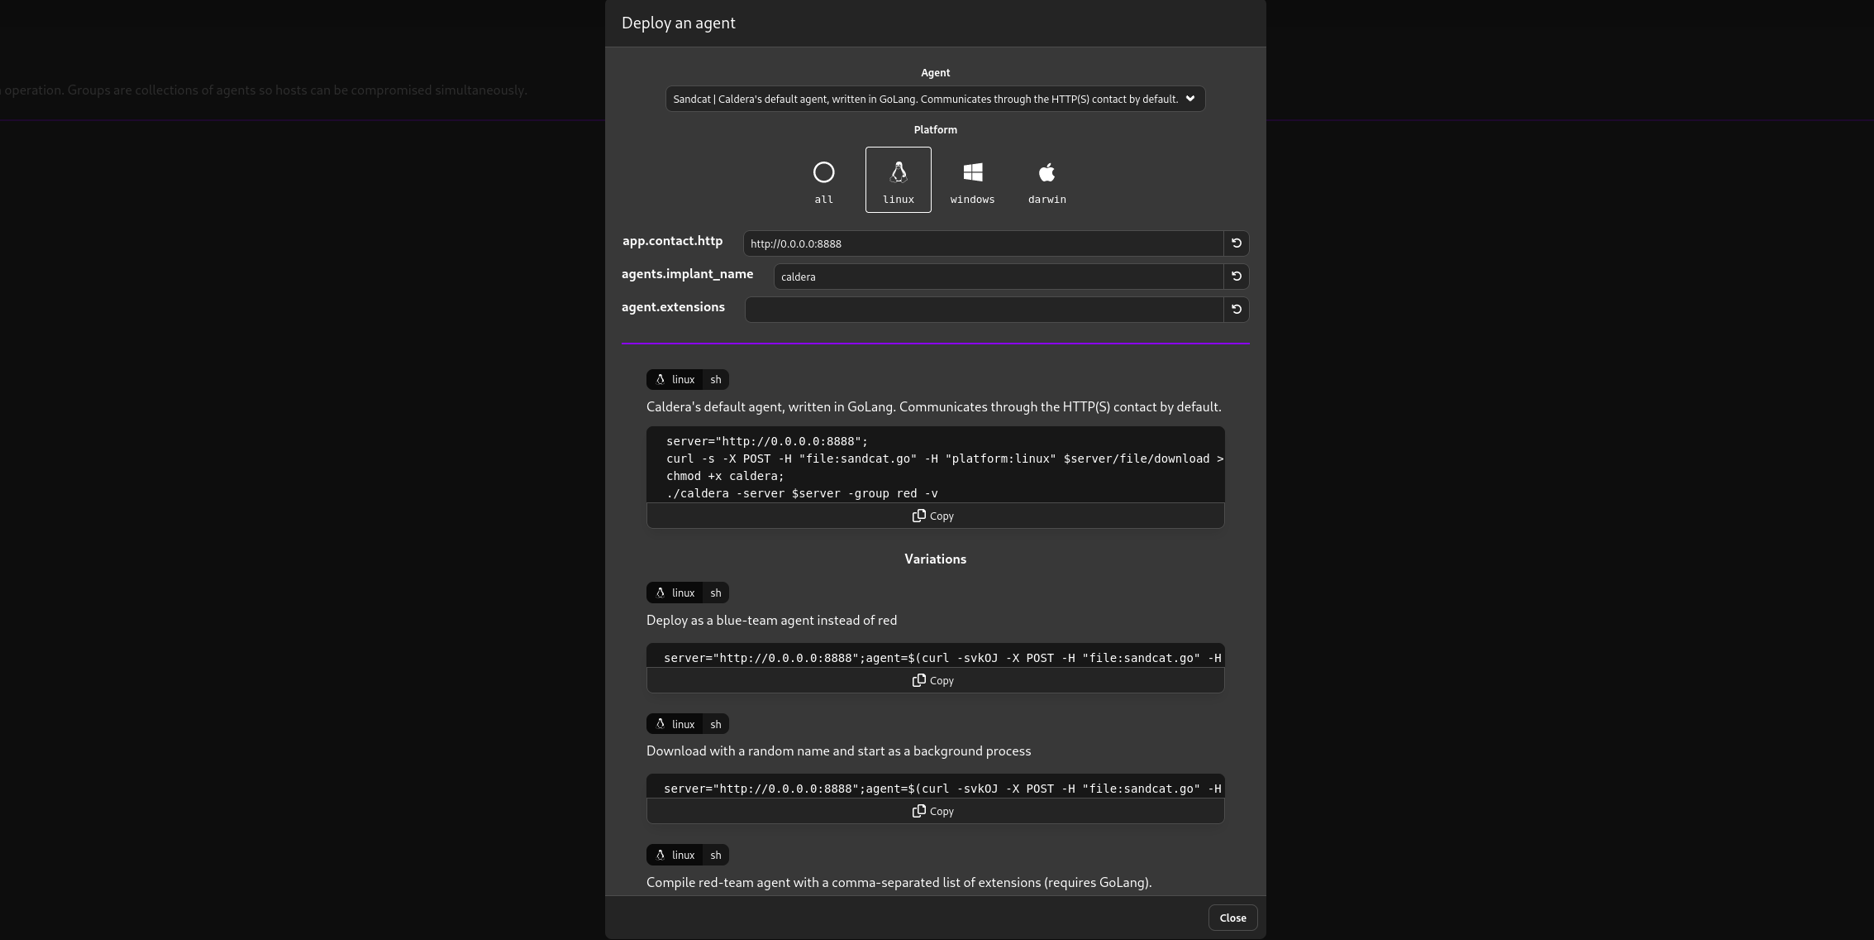
\includegraphics[width=1\linewidth]{imagenes/caldera-agent-v2.png}
    \caption{Proceso de configuración de un agente de \gls{CALDERA}}
    \label{fig:caldera-agents}
\end{figure}

En este caso, las máquinas víctima son contenedores de Ubuntu Server, por ello se hará uso de la plataforma Linux y del agente recomendado por defecto: Sandcat, que realiza las comunicaciones por medio del protocolo \texttt{\gls{HTTP}(s)}.

\begin{figure}[H]
    \centering
    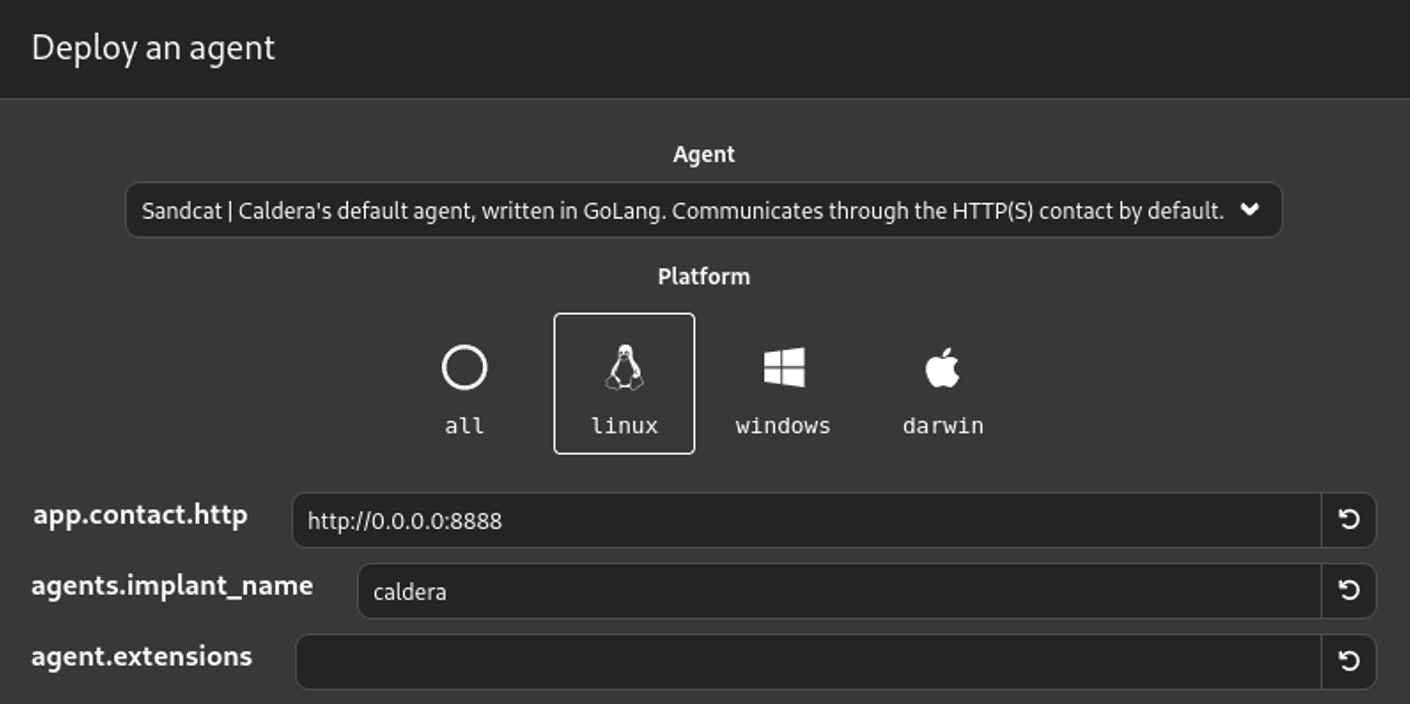
\includegraphics[width=1\linewidth]{imagenes/sandcat-agent.png}
    \caption{Selección del agente Sandcat para la infección de las máquinas víctima}
    \label{fig:sandcat-agent}
\end{figure}

Una vez obtenido el \textit{payload} que se va a utilizar simplemente es necesario ejecutarlo en la línea de comandos de cada una de las máquinas infectadas, y ya se creará el túnel por el cual se enviarán el resto de comandos a esta.

\begin{figure}[H]
    \centering
    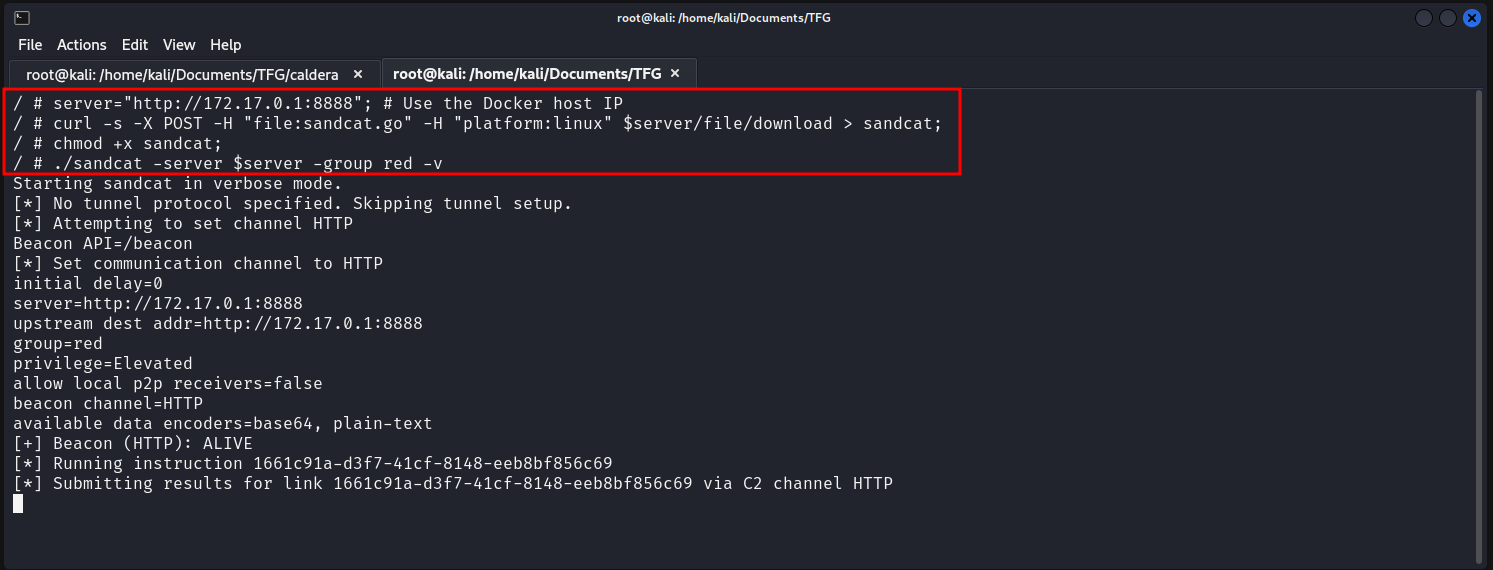
\includegraphics[width=1\linewidth]{imagenes/ejecucion-payload.png}
    \caption{Ejecución del \textit{payload} para generar un agente conectado a la máquina}
    \label{fig:ejecucion-payload}
\end{figure}

Es entonces cuando aparecerá un nuevo agente en la interfaz web con la siguiente información:

\begin{table}[H]
\centering
\footnotesize
\label{tab:caldera-agent}
\begin{tabularx}{\textwidth}{|X|X|X|X|X|} 
\hline
\texttt{id(paw)} & \texttt{host} & \texttt{group} & \texttt{platform} & \texttt{contact} \\
\hline
\texttt{dsmzqo} & \texttt{de2297825335} & \texttt{red} & \texttt{linux} & \texttt{HTTP} \\
\hline 
\end{tabularx}

\vspace{2mm}

\begin{tabularx}{\textwidth}{|X|X|X|X|}
\hline
\texttt{pid} & \texttt{privilege} & \texttt{status} & \texttt{last seen}  \\
\hline
\texttt{66} & \texttt{Elevated} & \texttt{alive, trusted} & \texttt{4/29/2024, 7:02:13 PM}\\
\hline 
\end{tabularx}
\caption{Formato de la tabla de un agente de CALDERA}
\end{table}

Una vez es posible visualizar dicho contenido, significa que los agentes han sido correctamente creados, y si el valor del campo \texttt{status} es \texttt{alive, trusted} significa que estos están preparados para adquirir habilidades, asignarlas a adversarios y posteriormente llevar a cabo las operaciones, es decir, los ataques.

\begin{figure}[H]
    \centering
    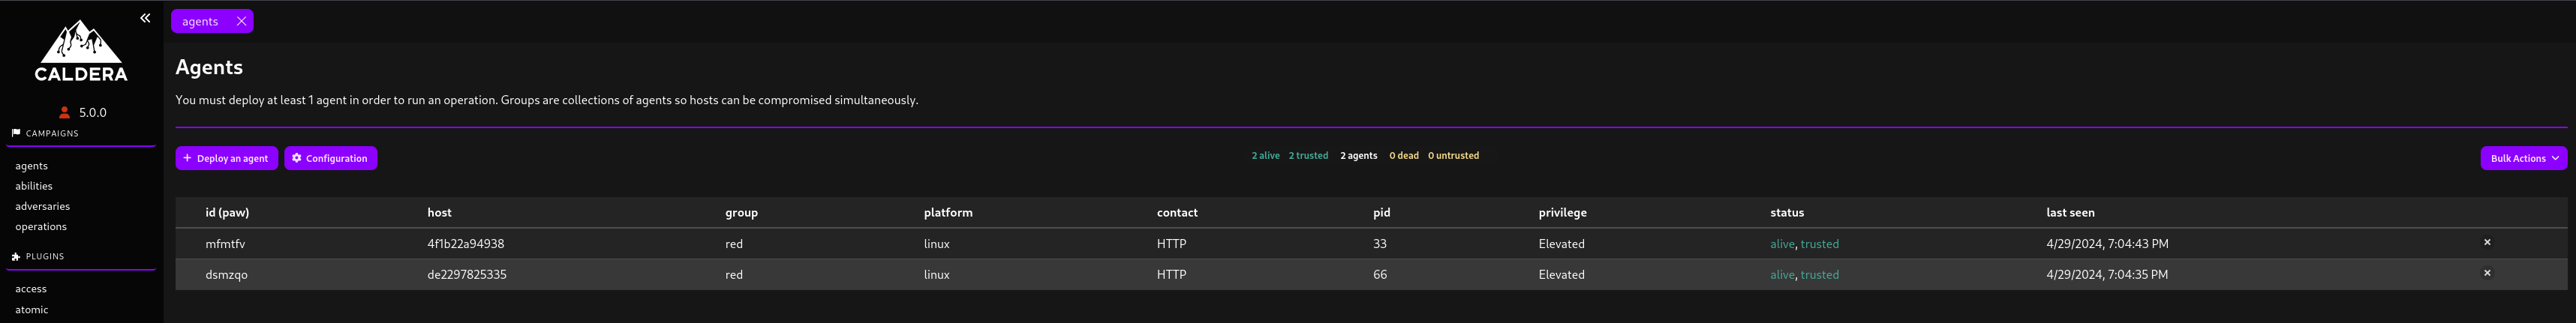
\includegraphics[width=1\linewidth]{imagenes/prepared-agents.png}
    \caption{Verificación del estado de los agentes configurados}
    \label{fig:prepared-agents}
\end{figure}

El siguiente paso es seleccionar aquellas habilidades que se quieran utilizar para las operaciones. Estas están directamente conectadas al marco de MITRE \gls{ATT&CK}, por lo que se dispone de una gran cantidad de \gls{TTP}s, concretamente más de 1600 habilidades. Además, es posible filtrar mediante una barra de búsqueda en función del tipo de táctica, técnica o procedimiento que se quiera utilizar, ya sea a través de lenguaje natural o bien mediante los códigos de identificación mencionados en el tercer capítulo \ref{tab:mitre_attack_matrices}. Además, también existe la posibilidad de agrupar un conjunto de habilidades bajo un identificador especificado manualmente, y posteriormente asignar dicho conjunto a un adversario.

\begin{figure}[H]
    \centering
    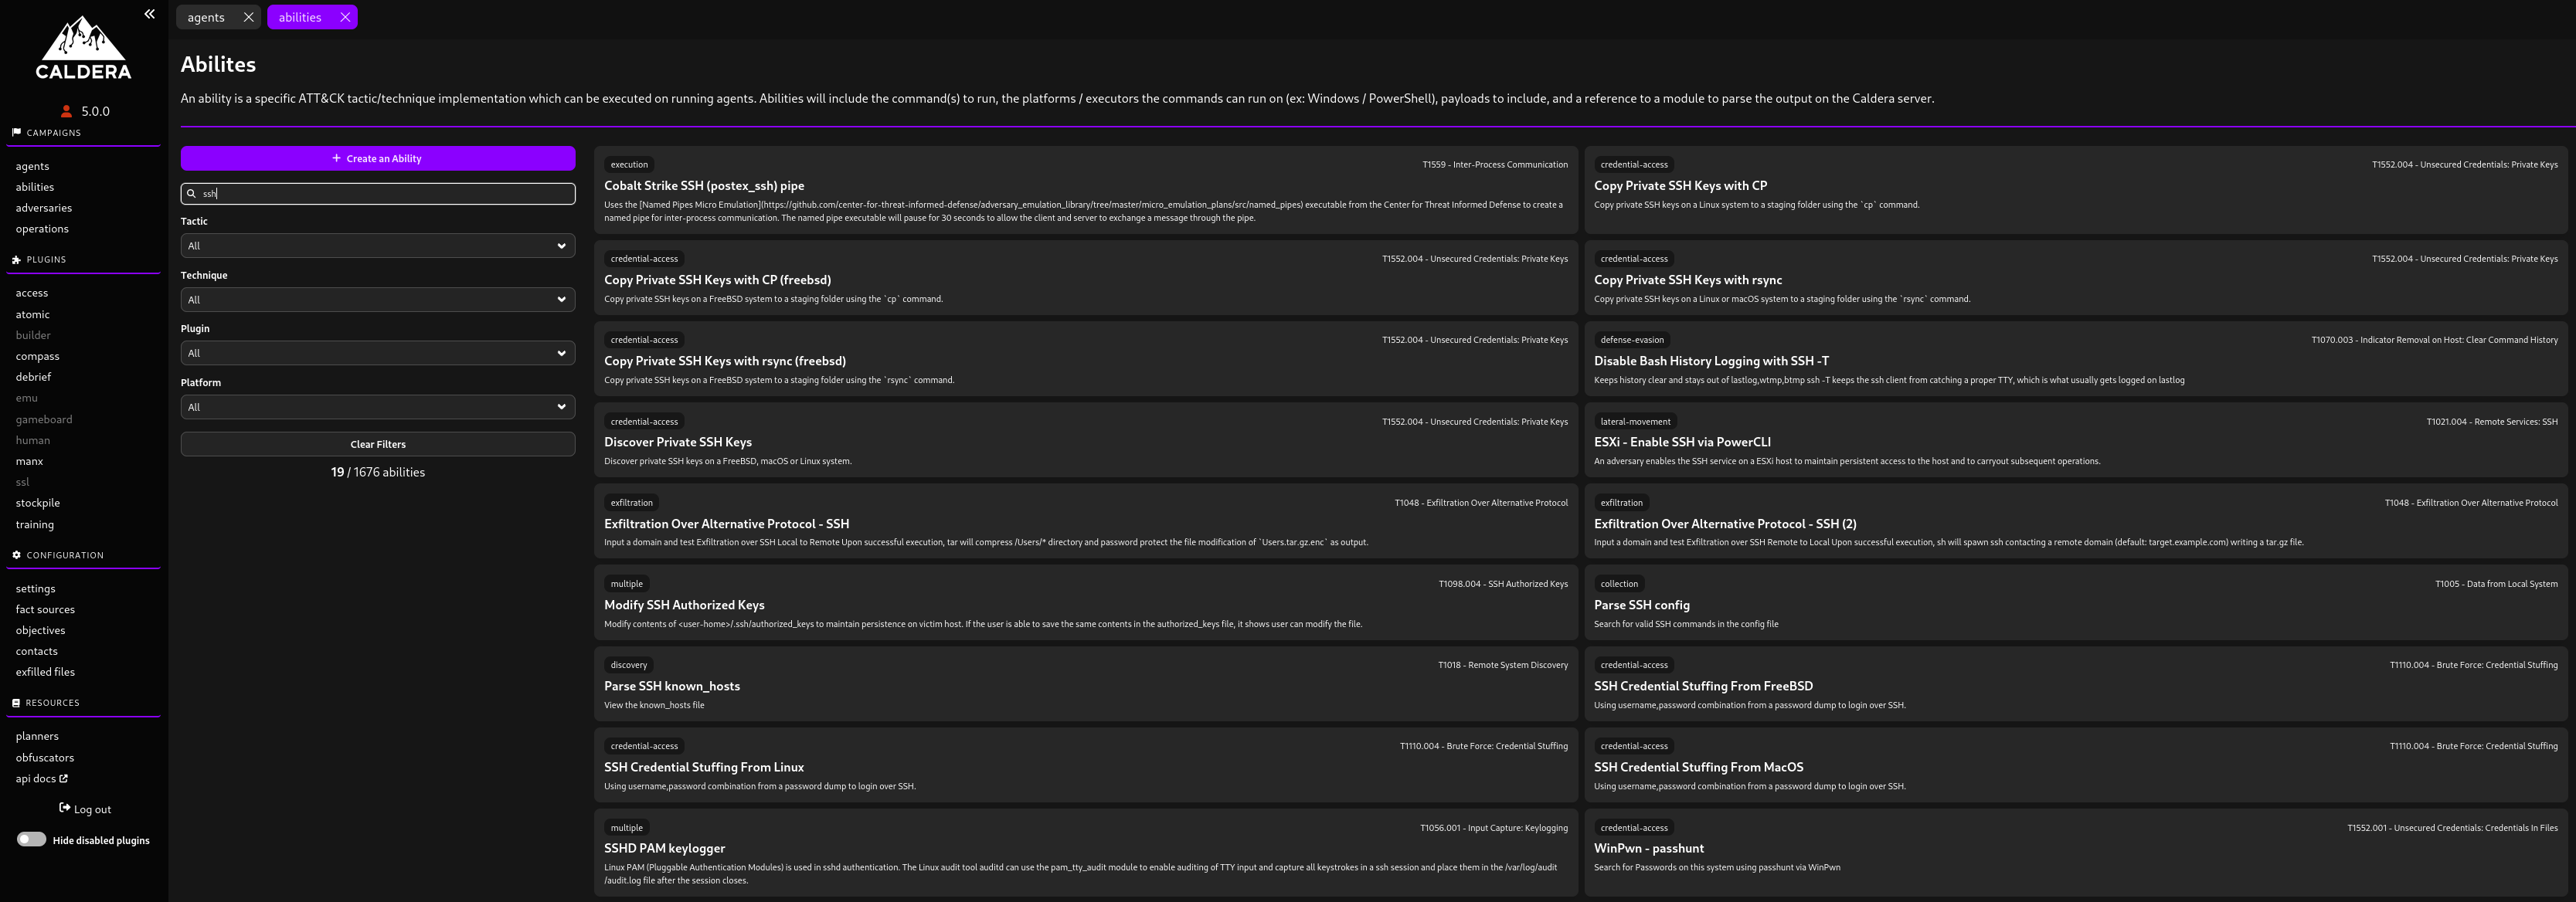
\includegraphics[width=1\linewidth]{imagenes/abilities-caldera.png}
    \caption{Ejemplo de filtrado en el panel de navegación de habilidades de \gls{CALDERA}}
    \label{fig:abilities-caldera}
\end{figure}

En tercer lugar, accediendo en el menú de navegación a la sección de adversarios debe seleccionarse entre las opciones del desplegable para crear un nuevo perfil, o bien importarlo a partir de un fichero.

\begin{figure}[H]
    \centering
    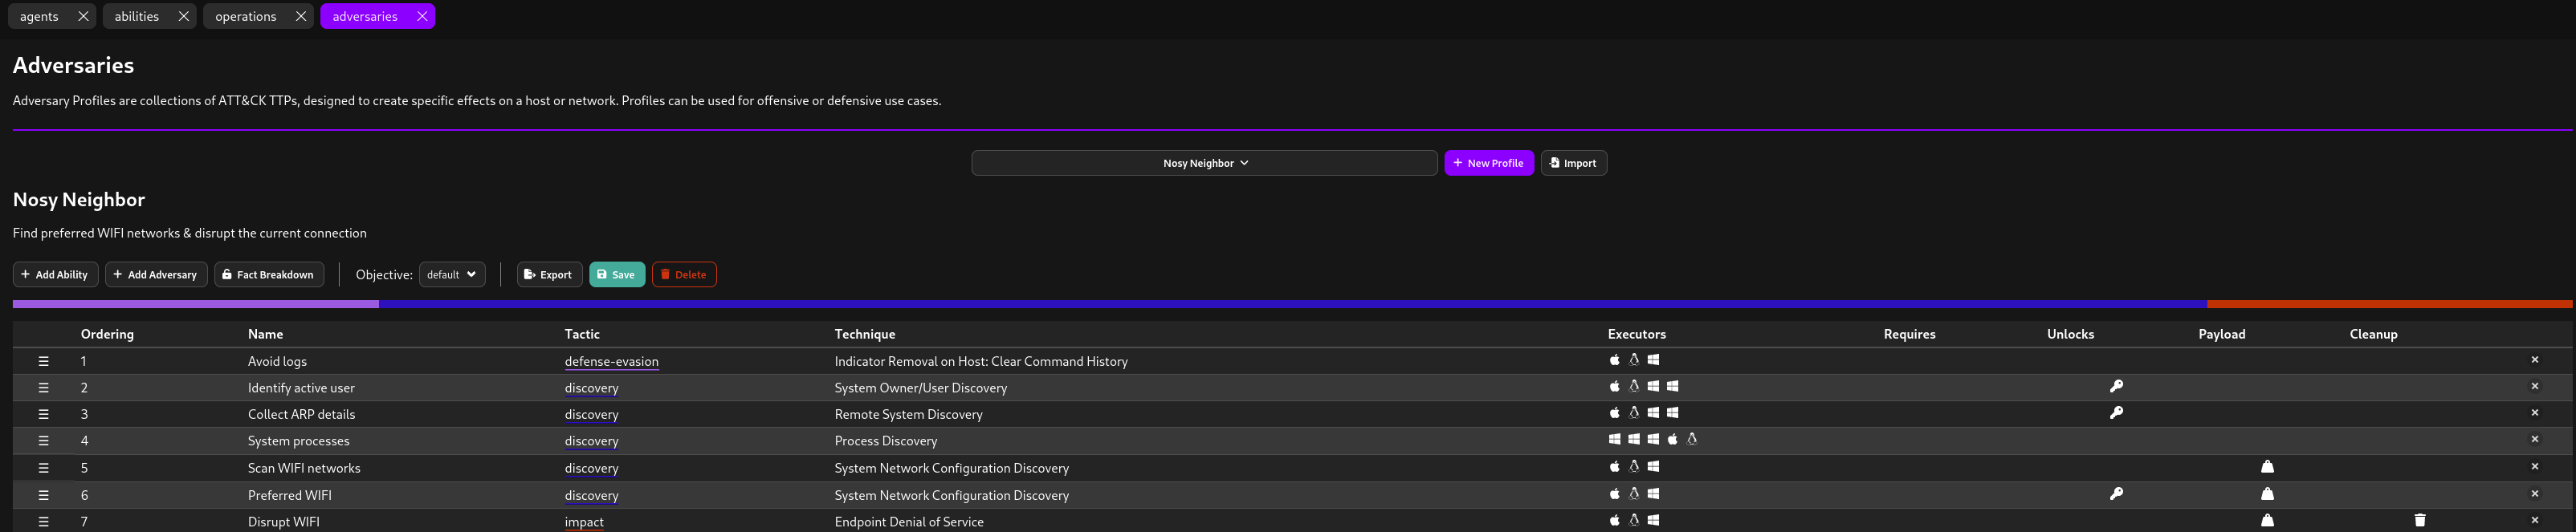
\includegraphics[width=1\linewidth]{imagenes/caldera-adversaries.png}
    \caption{Configuración de un perfil de adversario en \gls{CALDERA}}
    \label{fig:enter-label}
\end{figure}

Por último, para crear una nueva operación es necesario acceder a través del panel lateral y posteriormente hacer click en el botón de \texttt{+ New Operation}. Aparecerá una ventana donde se podrán rellenar campos de interés como el nombre de la operación, el adversario utilizado (lo más importante), grupo al que pertenece, métodos de ofuscación (por defecto las operaciones se lanzan en texto plano salvo que se seleccione lo contrario) y otras opciones de personalización adicionales.

\begin{figure}[H]
    \centering
    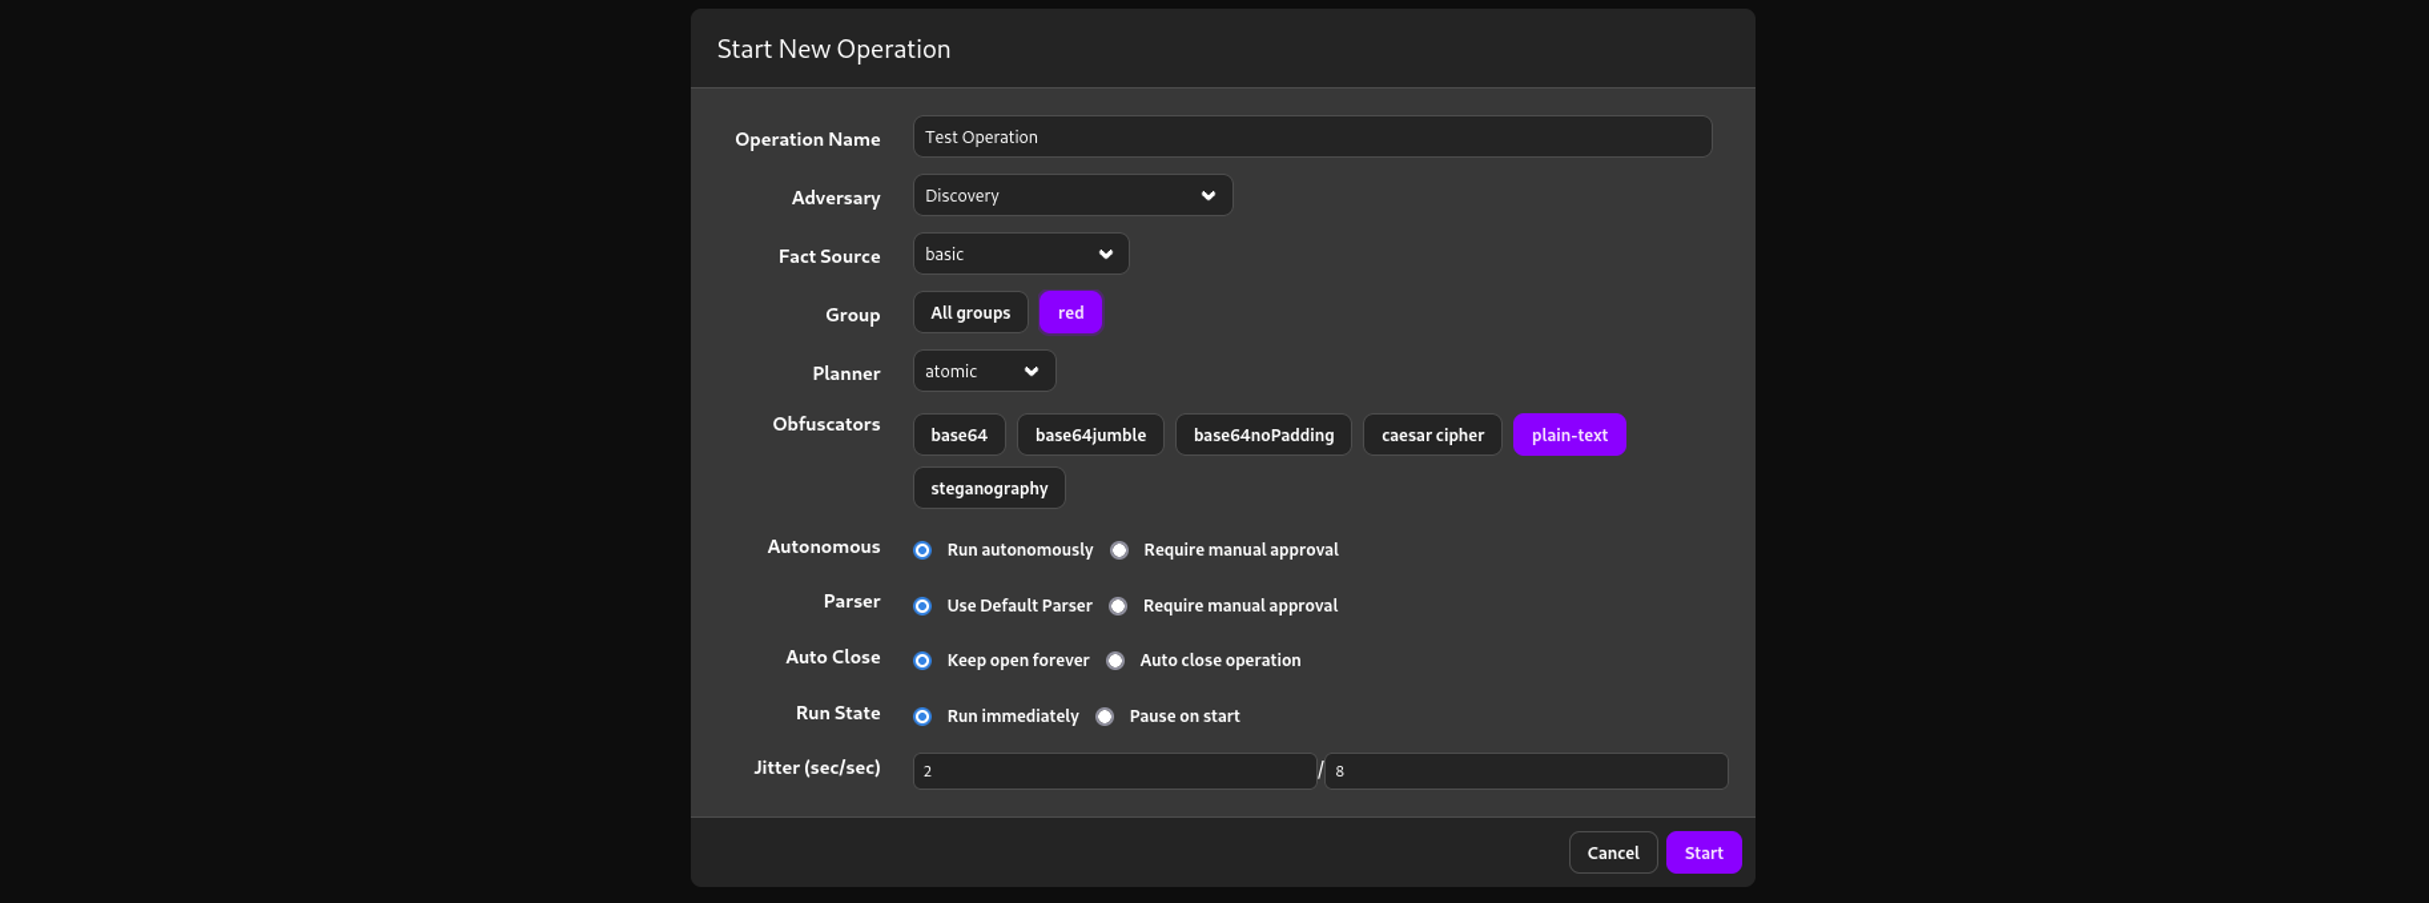
\includegraphics[width=1\linewidth]{imagenes/caldera-operation.png}
    \caption{Configuración de una operación de caldera a partir de un perfil adversario}
    \label{fig:caldera-operation}
\end{figure}

